\documentclass{../khlslides}

\usetikzlibrary{arrows.meta}

\title[Fundamenten]{Fundamenten}
\author{Fr\'ed\'eric Vogels}



\begin{document}

\begin{frame}
  \titlepage
\end{frame}

\begin{frame}
  \frametitle{Wat is een Computer?}
  \begin{center}
    \begin{tikzpicture}[node/.style={fill=blue!60,minimum size=1cm,opacity=.75,text opacity=1,drop shadow},
                        arc/.style={blue!75,ultra thick},
                        -->/.style={-latex,arc},
                        <--/.style={latex-,arc},
                        <-->/.style={latex-latex,arc}
                       ]
      
      \only<1>{
        \node {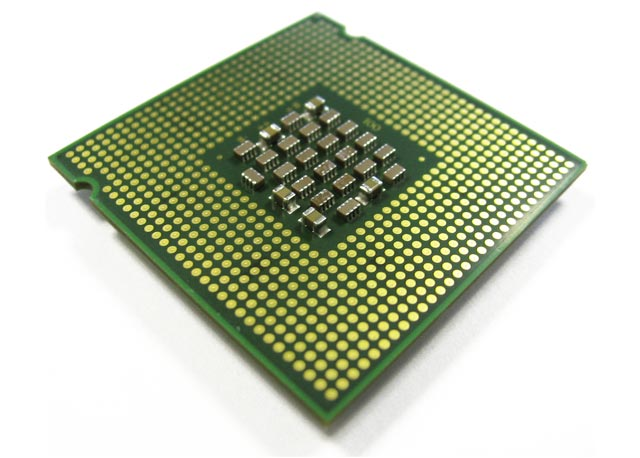
\includegraphics[width=10cm]{cpu.jpg}};
      }

      \only<2>{
        \node[opacity=.5] {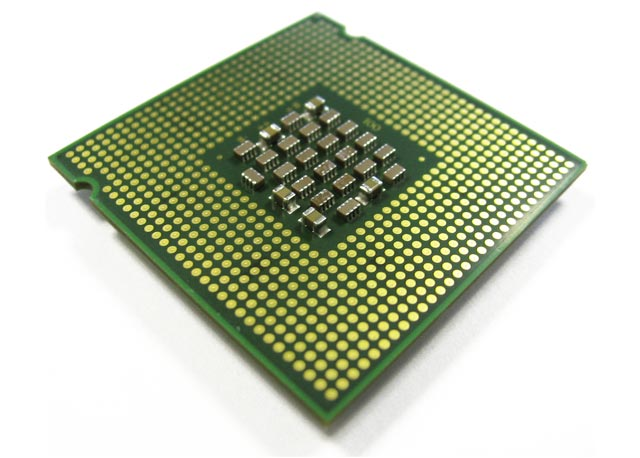
\includegraphics[width=10cm]{cpu.jpg}};

        \foreach[count=\i] \c in {toetsenbord,muis,netwerk,geluidskaart,gpu,printer} {
          \pgfmathparse{\i*60}\let\angle\pgfmathresult
          \node[node] (\c) at (\angle:3.5cm) {\c};
        }

        \node[node,minimum width=2cm] (cpu) {\sc\Huge cpu};

        \draw[-->] (muis) -- (cpu);
        \draw[-->] (toetsenbord) -- (cpu);
        \draw[<--] (printer) -- (cpu);
        \draw[<--] (gpu) -- (cpu);
        \draw[<--] (geluidskaart) -- (cpu);
        \draw[<-->] (netwerk) -- (cpu);
      }
    \end{tikzpicture}
  \end{center}
\end{frame}

\begin{frame}
  \frametitle{Wat is een Computer?}
  \begin{center}
    \begin{tikzpicture}[node/.style={fill=blue!60,minimum size=1cm,opacity=.75,text opacity=1,drop shadow},
                        arc/.style={blue!75,ultra thick,-latex},]
      \node[node] (cpu) {\sc\Huge cpu};
      \draw[arc] ($ (cpu.west) + (-3,0) $) -- (cpu.west)
                 node[midway,above] {input}
                 node[midway,below] {\color{black}\tiny\tt10110110110101111};
      \draw[arc] (cpu.east) -- ($ (cpu.east) + (3,0) $)
                 node[midway,above] {output}
                 node[midway,below] {\color{black}\tiny\tt00101101110101010};

      \node[/khl/note] (note) at ($ (cpu.south) + (0,-2) $) {Veredelde rekenmachine};
      \draw[/khl/note arrow] (note) -- (cpu);      
    \end{tikzpicture}
  \end{center}
\end{frame}

\begin{frame}
  \frametitle{Cijfertjes}
  \begin{center} \small
    \begin{tabular}{llll}
      Jaar & Platform & \$/GFLOP & GFLOP \\
      \toprule
      1961 & \NODE{IBM 1620}{ibm 1620} & 8,300,000,000,000 \\
      1984 & Cray X-MP/48 & 42,780,000 & 0.8 \\
      2000 & Playstation 2 & 63.2 & 6.2 \\
      2006 & Playstation 3 & 2.35 & 230.4 \\
      2011 & HPU4Science & 1.80 & 20,000 \\
      2013 & Playstation 4 & 0.22 & 1840 \\
      2014 & Sempron 145 + GTX 760 & 0.16 & 6771 \\
    \end{tabular}
  \end{center}
  \begin{tikzpicture}[overlay,remember picture]
    \only<2>{
      \node[/khl/note,anchor=south] (note ibm 1620) at ($ (ibm 1620) + (1,1) $) {\parbox{6cm}{\raggedright Voerde 50 vermenigvuldigingen per seconden uit!}};
      \draw[/khl/note arrow] (note ibm 1620) -- (ibm 1620);
    }
  \end{tikzpicture}
\end{frame}

\begin{frame}
  \frametitle{Operaties op Getallen}
  \begin{center}
    \begin{tabular}{cl}
      {\bf Operator} & {\bf Beschrijving} \\
      \toprule
      {\tt a + b} & Optelling \\
      {\tt a - b} & Aftrekking \\
      {\tt a * b} & Vermenigvuldiging \\
      {\tt a / b} & Deling \\
      {\tt a \% b} & Rest bij deling \\
      {\tt Math.pow(a, b)} & Machtsverheffing \\
      {\tt Math.sqrt(a)} & Vierkantswortel \\[2mm]
      {\tt \^{}} & \alert{Niet} de machtsverheffing \\
    \end{tabular}
  \end{center}
\end{frame}

\begin{frame}
  \frametitle{Expressies}
  \begin{itemize}
    \item Expressies worden stap voor stap ge\"evalueerd
    \item Expressies leiden uiteindelijk tot een waarde
  \end{itemize}

  \vskip5mm
  \structure{Voorbeeld van stapsgewijze evaluatie}

  \begin{center}
    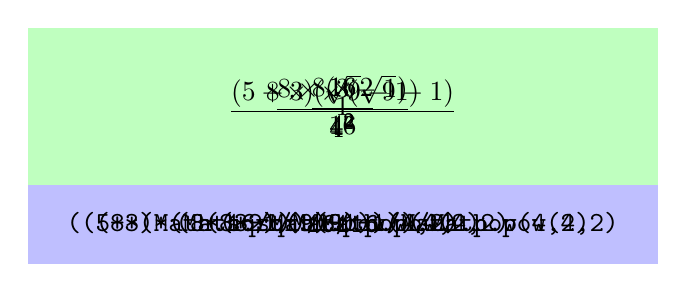
\begin{tikzpicture}
      \path[fill=green!25] (-4,-1) rectangle (4, 1);
      \path[fill=blue!25] (-4,-1) rectangle (4, -2);

      \visible<1>{
        \node {$\displaystyle \frac{ (5+3) \times (\sqrt9-1)}{4^2}$};
        \node at (0,-1.5) {\tt ((5+3)*(Math.sqrt(9)-1))/Math.pow(4,2)};
      }      

      \visible<2>{
        \node {$\displaystyle \frac{ 8 \times (\sqrt9-1)}{4^2}$};
        \node at (0,-1.5) {\tt (8*(Math.sqrt(9)-1))/Math.pow(4,2)};
      }      

      \visible<3>{
        \node {$\displaystyle \frac{ 8 \times (3-1)}{4^2}$};
        \node at (0,-1.5) {\tt (8*(3-1))/Math.pow(4,2)};
      }      

      \visible<4>{
        \node {$\displaystyle \frac{8\times 2}{4^2}$};
        \node at (0,-1.5) {\tt (8*2)/Math.pow(4,2)};
      }      

      \visible<5>{
        \node {$\displaystyle \frac{16}{4^2}$};
        \node at (0,-1.5) {\tt 16/Math.pow(4,2)};
      }      

      \visible<6>{
        \node {$\displaystyle \frac{16}{16}$};
        \node at (0,-1.5) {\tt 16/16};
      }      

      \visible<7>{
        \node {$\displaystyle 1$};
        \node at (0,-1.5) {\tt 1};
      }      
    \end{tikzpicture}
  \end{center}
\end{frame}

\begin{frame}
  \frametitle{Probleem}
  \[
    a \cdot x^2 + b \cdot x + c = 0
  \]
  heeft als oplossingen
  \[
    x_1 = \frac{-b-\sqrt{b^2-4 \cdot a\cdot c}}{2 \cdot a}
    \qquad
    x_2 = \frac{-b+\sqrt{b^2-4 \cdot a\cdot c}}{2 \cdot a}
  \]
  \vskip4mm
  \begin{itemize}
    \item Vrij onoverzichtelijk
    \item Deelexpressie $\sqrt{b^2-4 \cdot a\cdot c}$ wordt $2\times$ uitgevoerd
  \end{itemize}
\end{frame}

{
  \newcommand{\STEP}[1]{
    \onslide<#1>
    \code[width=.95\linewidth,font size=\small]{quadratic#1.js}
  }
  \begin{frame}
    \frametitle{Variabelen}
    \structure{Variabelen}
    \begin{itemize}
      \item We kunnen resultaten bewaren in \emph{variabelen}
      \item Variabelen krijgen een naam mee
      \item Leesbaarder \& effici\"enter
    \end{itemize}
    \vskip4mm
    \structure{Voorbeeld}
    \[ x^2+x-6=0 \]
    \begin{overprint}
      \STEP1
      \STEP2
      \STEP3
      \STEP4
      \STEP5
      \STEP6
      \STEP7
      \STEP8
      \STEP9
      \STEP{10}
      \STEP{11}
      \STEP{12}
      \STEP{13}
      \STEP{14}
      \STEP{15}
      \STEP{16}
      \STEP{17}
      \STEP{18}
      \STEP{19}
      \STEP{20}
      \STEP{21}
      \STEP{22}
    \end{overprint}
  \end{frame}
}

\begin{frame}
  \frametitle{Variabelen}
  \begin{overprint}
    \onslide<1-2>
    \code[width=.2\linewidth,font size=\small]{vars1.js}

    \onslide<3>
    \code[width=.2\linewidth,font size=\small]{vars2.js}

    \onslide<4>
    \code[width=.2\linewidth,font size=\small]{vars3.js}
  \end{overprint}
  \begin{tikzpicture}[overlay,remember picture]
    \only<1>{
      \node[/khl/note,anchor=south west] (note declaration) at ($ (declaration) + (1,1) $) {Declaratie};
      \draw[/khl/note arrow] (note declaration) -- (declaration.north east);
    }

    \only<2>{
      \node[/khl/note,anchor=south west] (note initialization) at ($ (initialization) + (1,1) $) {Toekenning};
      \draw[/khl/note arrow] (note initialization) -- (initialization.north east);
    }

    \only<3>{
      \node[/khl/note,anchor=south west] (note combination) at ($ (combination) + (1,1) $) {Declaratie + initialisatie};
      \draw[/khl/note arrow] (note combination) -- (combination.north east);
    }
  \end{tikzpicture}
  \begin{overprint}
    \onslide<1>
    Een \emph{declaratie} voert een nieuwe variabele in. De computer zoekt een stukje vrij geheugen en geeft dit een naam.

    \onslide<2>
    Een \emph{toekenning} kent een waarde toe aan een variabele. De eerste toekenning wordt vaak ook
    \emph{initialisatie} genoemd.

    \onslide<3>
    Een variabele kan bij declaratie meteen ge\"initialiseerd worden.

    \onslide<4>
    Dit is fout: {\tt x} heeft geen waarde.
  \end{overprint}
\end{frame}


\begin{frame}
  \frametitle{Toekenningen}
  Variabelen zijn overschrijfbaar:
  \vskip1cm
  \code[width=.3\linewidth]{overwrite.js}
  \begin{tikzpicture}[overlay,remember picture]
    \only<1>{
      \node[/khl/note,anchor=south west] (init note) at ($ (init) + (1,1) $) {{\tt x} wordt ge\"initialiseerd op {\tt 5}};
      \draw[/khl/note arrow] (init note) -- (init.north east);
    }

    \only<2>{
      \node[/khl/note,anchor=south west] (assignment note) at ($ (assignment) + (1,1) $) {{\tt x} wordt overschreven met {\tt 3}};
      \draw[/khl/note arrow] (assignment note) -- (assignment.north east);
    }

    \only<3>{
      \node[/khl/note,anchor=south west] (rhs note) at ($ (rhs) + (1,1) $) {\parbox{5cm}{\raggedright Rechterlid wordt eerst ge\"evalueerd}};
      \draw[/khl/note arrow] (rhs note) -- (rhs.north east);
    }

    \only<4>{
      \node[/khl/note] (lhs note) at ($ (lhs) + (-1,-1) $) {Resultaat ({\tt 6}) wordt toegekend aan {\tt x}};
      \draw[/khl/note arrow] (lhs note) -- (lhs.south west);
    }
  \end{tikzpicture}
\end{frame}


\begin{frame}
  \frametitle{Toekenningen: Oefening}
  Welke waarden steken er in de variabelen {\tt x} en {\tt y}?
  \vskip1cm
  \code[width=.3\linewidth]{assign-exercise.js}
  \begin{tikzpicture}[overlay,remember picture]
    \only<2>{
      \node[/khl/note,anchor=west] (first note) at ($ (first) + (2,0) $) {\parbox{1cm}{{\tt x} = 5}};
      \draw[/khl/note arrow] (first note) -- (first.east);
    }

    \only<3>{
      \node[/khl/note,anchor=west] (second note) at ($ (second) + (2,0) $) {
        \parbox{1cm}{{\tt x} = 5 \\ {\tt y} = 5}
      };
      \draw[/khl/note arrow] (second note) -- (second.east);
    }

    \only<4>{
      \node[/khl/note,anchor=west] (third note) at ($ (third) + (2,0) $) {
        \parbox{1.2cm}{{\tt x} = 10 \\ {\tt y} = 5}
      };
      \draw[/khl/note arrow] (third note) -- (third.east);
    }
  \end{tikzpicture}
\end{frame}


\begin{frame}
  \frametitle{Speciale Notaties}
  \begin{center}
    \begin{tabular}{l@{\hspace{1cm}}l}
      {\bf Notatie} & {\bf Betekenis} \\
      \toprule
      {\tt x += y} & {\tt x = x + y} \\
      {\tt x -= y} & {\tt x = x - y} \\
      {\tt x *= y} & {\tt x = x * y} \\
      {\tt x /= y} & {\tt x = x / y} \\
      {\tt x \%= y} & {\tt x = x \% y} \\[2mm]
      {\tt ++x} of {\tt x++} & {x = x + 1} \\
      {\tt --x} of {\tt x--} & {x = x - 1} \\
    \end{tabular}
  \end{center}
\end{frame}


\begin{frame}
  \frametitle{Basiselementen van Algoritmes}
  Algoritmes bestaat uit een reeks basiselementen:
  \vskip2mm
  \begin{itemize}
    \item Basisberekeningen {\tt +}, {\tt -}, {\tt *}, {\tt /}, \dots \vskip2mm
    \item Sequentie: berekeningen die elkaar opvolgen \vskip2mm
    \item Selectie: berekeningen overslaan naargelang een conditie \vskip2mm
    \item Iteratie: herhalen van bepaalde berekeningen
  \end{itemize}
\end{frame}


\begin{frame}
  \frametitle{Vergelijken van Getallen}
  \begin{center}
    \begin{tabular}{cl}
      {\bf Operator} & {\bf Beschrijving} \\
      \toprule
      {\tt ===} & Gelijk aan \\
      {\tt !==} & Niet gelijk aan \\
      {\tt <} & Kleiner dan \\
      {\tt <=} & Kleiner dan of gelijk aan \\
      {\tt >} & Groter dan \\
      {\tt >=} & Groter dan of gelijk aan \\
    \end{tabular}
  \end{center}
\end{frame}


{
  \newcommand{\STEP}[1]{
    \onslide<#1>
    \code[width=.3\linewidth,font size=\small]{comparison#1.js}
  }
  \begin{frame}
    \frametitle{Booleans}
    \structure{Voorbeeld}
    \vskip2mm
    \begin{overprint}
      \STEP1
      \STEP2
      \STEP3
      \STEP4
      \STEP5
      \STEP6
    \end{overprint}
  \end{frame}
}

\begin{frame}
  \frametitle{Booleans}
  \begin{itemize}
    \item Booleans drukken waarheidswaarden uit
          \begin{itemize}
            \item {\tt true}
            \item {\tt false}
          \end{itemize}
    \item Zijn het resultaat van vergelijkingen {\tt ===}, {\tt !==}, {\tt <}, \dots
    \item Hebben hun eigen operatoren
  \end{itemize}
  \begin{center}
    \begin{tabular}{cl}
      {\bf Operator} & {\bf Beschrijving} \\
      \toprule
      {\tt \&\&} & Conjunctie (en) \\
      {\tt ||} & Disjunctie (of) \\
      {\tt !} & Negatie (niet) \\
    \end{tabular}
  \end{center}
\end{frame}

{
  \newcommand{\STEP}[1]{
    \onslide<#1>
    \code[width=.55\linewidth,font size=\small]{conj-example#1.js}
  }

  \begin{frame}
    \frametitle{Conjunctie (en)}
    \begin{center}
      \begin{tabular}{ccc}
        {\tt\bfseries a} & {\tt\bfseries b} & {\tt\bfseries a \&\& b} \\
        \toprule
        {\tt false} & {\tt false} & {\tt false} \\
        {\tt false} & {\tt true} & {\tt false} \\
        {\tt true} & {\tt false} & {\tt false} \\
        {\tt true} & {\tt true} & {\tt true} \\
      \end{tabular}
    \end{center}

    \vskip4mm

    \structure{Voorbeeld}
    \begin{overprint}
      \STEP1
      \STEP2
      \STEP3
      \STEP4
      \STEP5
      \STEP6
    \end{overprint}
  \end{frame}
}

\begin{frame}
  \frametitle{Andere Logische Operatoren}
  \structure{Disjunctie (of)}
  \begin{center}
    \begin{tabular}{ccc}
      {\tt\bfseries a} & {\tt\bfseries b} & {\tt\bfseries a || b} \\
      \toprule
      {\tt false} & {\tt false} & {\tt false} \\
      {\tt false} & {\tt true} & {\tt true} \\
      {\tt true} & {\tt false} & {\tt true} \\
      {\tt true} & {\tt true} & {\tt true} \\
    \end{tabular}
  \end{center}

  \vskip5mm

  \structure{Negatie (niet)}
  \begin{center}
    \begin{tabular}{ccc}
      {\tt\bfseries a} & {\tt\bfseries !a} \\
      \toprule
      {\tt false} & {\tt true} \\
      {\tt true} & {\tt false} \\
    \end{tabular}
  \end{center}
\end{frame}

{
  \newcommand{\STEP}[1]{
    \onslide<#1>
    \code[width=.3\linewidth,font size=\small]{ltlt#1.js}
  }

  \begin{frame}
    \frametitle{Veelgemaakte Fout}
    \structure{Tot wat evalueert de volgende expressie?}
    \vskip4mm
    \begin{overprint}
      \STEP1
      \STEP2

      \onslide<3->
      \code[width=.3\linewidth,font size=\small]{ltlt3.js}
    \end{overprint}
    \visible<4>{
      \begin{itemize}
        \item Typefout!
        \item Men kan een boolean niet vergelijken ({\tt <}) met een getal
        \item Juiste manier: {\tt 3 < 5 \&\& 5 < 8}
        \item Idem voor andere operatoren
              \begin{itemize}
                \item {\tt a === b \&\& b === c}
                \item {\tt a > b \&\& b > c}
                \item \dots
              \end{itemize}
      \end{itemize}
    }
  \end{frame}
}

\begin{frame}
  \frametitle{Shortcircuiting}
  \structure{Tot wat evalueert de volgende expressie?}
  \vskip4mm
  \begin{overprint}
    \onslide<1>
    \code[width=.41\linewidth,font size=\small]{shortcircuit1.js}

    \onslide<2>
    \code[width=.41\linewidth,font size=\small]{shortcircuit2.js}

    \onslide<3>
    \code[width=.41\linewidth,font size=\small]{shortcircuit3.js}
  \end{overprint}
  \begin{itemize}
    \item Problematische rechteroperand
          \begin{itemize}
            \item Deling 0 door 0: mag niet
            \item Vergelijking tussen getal en 
          \end{itemize}
    \item Shortcircuiting
          \begin{itemize}
            \item {\tt false \&\& b} zal altijd {\tt false} opleveren
            \item Moeite wordt niet gedaan om rechteroperand te evalueren
          \end{itemize}
  \end{itemize}
  \visible<2->{
    \begin{center}
      \begin{tabular}{ccc}
        {\tt\bfseries a} & {\tt\bfseries b} & {\tt\bfseries a \&\& b} \\
        \toprule
        {\tt false} & {\tt false} & {\tt false} \\
        {\tt false} & {\tt true} & {\tt false} \\
        {\tt true} & {\tt false} & {\tt false} \\
        {\tt true} & {\tt true} & {\tt true} \\
      \end{tabular}
    \end{center}
  }
\end{frame}


\begin{frame}
  \frametitle{Shortcircuiting}
  \begin{itemize}
    \item Minimaal aantal operanden wordt ge\"evalueerd
    \item {\tt true || b} leidt meteen tot {\tt true}
    \item {\tt false \&\& b} leidt meteen tot {\tt false}
    \item Shortcircuiting \emph{enkel} met {\tt \&\&} en {\tt ||}
    \item {\tt 0 * (0/0)} crasht dus wel!
  \end{itemize}
\end{frame}


\end{document}



%%% Local Variables: 
%%% mode: latex
%%% TeX-master: t
%%% End: 
